\documentclass[color=usenames,dvipsnames]{beamer}\usepackage[]{graphicx}\usepackage[]{xcolor}
% maxwidth is the original width if it is less than linewidth
% otherwise use linewidth (to make sure the graphics do not exceed the margin)
\makeatletter
\def\maxwidth{ %
  \ifdim\Gin@nat@width>\linewidth
    \linewidth
  \else
    \Gin@nat@width
  \fi
}
\makeatother

\definecolor{fgcolor}{rgb}{0.345, 0.345, 0.345}
\newcommand{\hlnum}[1]{\textcolor[rgb]{0.686,0.059,0.569}{#1}}%
\newcommand{\hlsng}[1]{\textcolor[rgb]{0.192,0.494,0.8}{#1}}%
\newcommand{\hlcom}[1]{\textcolor[rgb]{0.678,0.584,0.686}{\textit{#1}}}%
\newcommand{\hlopt}[1]{\textcolor[rgb]{0,0,0}{#1}}%
\newcommand{\hldef}[1]{\textcolor[rgb]{0.345,0.345,0.345}{#1}}%
\newcommand{\hlkwa}[1]{\textcolor[rgb]{0.161,0.373,0.58}{\textbf{#1}}}%
\newcommand{\hlkwb}[1]{\textcolor[rgb]{0.69,0.353,0.396}{#1}}%
\newcommand{\hlkwc}[1]{\textcolor[rgb]{0.333,0.667,0.333}{#1}}%
\newcommand{\hlkwd}[1]{\textcolor[rgb]{0.737,0.353,0.396}{\textbf{#1}}}%
\let\hlipl\hlkwb

\usepackage{framed}
\makeatletter
\newenvironment{kframe}{%
 \def\at@end@of@kframe{}%
 \ifinner\ifhmode%
  \def\at@end@of@kframe{\end{minipage}}%
  \begin{minipage}{\columnwidth}%
 \fi\fi%
 \def\FrameCommand##1{\hskip\@totalleftmargin \hskip-\fboxsep
 \colorbox{shadecolor}{##1}\hskip-\fboxsep
     % There is no \\@totalrightmargin, so:
     \hskip-\linewidth \hskip-\@totalleftmargin \hskip\columnwidth}%
 \MakeFramed {\advance\hsize-\width
   \@totalleftmargin\z@ \linewidth\hsize
   \@setminipage}}%
 {\par\unskip\endMakeFramed%
 \at@end@of@kframe}
\makeatother

\definecolor{shadecolor}{rgb}{.97, .97, .97}
\definecolor{messagecolor}{rgb}{0, 0, 0}
\definecolor{warningcolor}{rgb}{1, 0, 1}
\definecolor{errorcolor}{rgb}{1, 0, 0}
\newenvironment{knitrout}{}{} % an empty environment to be redefined in TeX

\usepackage{alltt}
%\documentclass[color=usenames,dvipsnames,handout]{beamer}

%\usepackage[roman]{../pres1}
\usepackage[sans]{../pres1}
\usepackage{graphicx}
\usepackage{bm}





\IfFileExists{upquote.sty}{\usepackage{upquote}}{}
\begin{document}



\begin{frame}[plain]
  \begin{center}
    {\huge Occupancy Estimation and Modeling \par}
    \vfill
    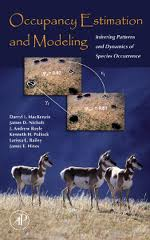
\includegraphics[height=4.6cm,keepaspectratio]{figs/book} %\hfill
    \hspace{0.5cm}
      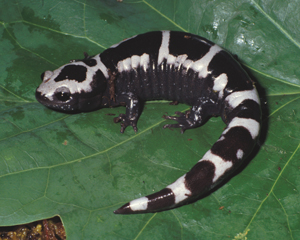
\includegraphics[height=4.6cm,keepaspectratio,trim = 0mm
        0mm 0mm 0mm, clip]{figs/marbled_salamander.jpg}
  \end{center}
\end{frame}



\section{Introduction}


\begin{frame}
  \frametitle{Motivation}
  {\centering \large Occupancy models were developed to estimate metapopulation
    parameters when \alert{detection probability} ($p$) is $<1$. \par}
  \pause
%  \Large
%  \[
%    \psi_{i,t+1} = O_{i,t}(1-\varepsilon) + (1-O_{i,t})\gamma
%  \]
%  \[
%    O_{i,t+1} \sim \mbox{Bernoulli}(\psi_{i,t+1})
%  \]
  \vspace{0.5cm}
  \large
  Parameters of interest:
  \begin{itemize}[<+->]
    \item $\psi$ -- Probability that a site is occupied
    \item $\gamma$ -- Probability that an unoccupied site becomes colonized
    \item $\varepsilon$ -- Probability that an occupied site goes extinct
    \item $p$ -- Probability of detecting at least one individual at a
      site that is occupied (on a single sampling occasion)
  \end{itemize}
\end{frame}




% \begin{frame}
%   \frametitle{Definitions}
%   In the context of occupancy models\dots \\
%   \begin{itemize}[<+->]
%     \item {\bf Detection probability}: the probability of detecting at
%       least one individual at a site during a sampling occasion, given
%       that species is present
%     \item {\bf Sampling occasion}
%     \item {\bf Occurrence probability}
%   \end{itemize}
% \end{frame}





\begin{frame}
  \frametitle{Detection probability}
  \large
  {\centering If $p<1$, we might
    incorrectly conclude that a site is unoccupied if we don't detect
    any individuals \par}
  \pause
  \vspace{0.5cm}
  {%\bf
    Consequences}
  \begin{itemize}[<+->]
    \item We will underestimate the state variable: The proportion of
      sites occupied
    \item We might make incorrect conclusions about habitat relationships
  \end{itemize}
\end{frame}







\section{Single-season models}




\begin{frame}
  \frametitle{Single-season models}
  \large
  {%\bf
    Scenario}
  \large
  \begin{itemize}[<+->]
    \item No interest in colonization or extinction events
    \item Instead, we directly estimate $\psi$ during one season
    \item Useful for assessing snapshot of habitat relationships or
      for modeling a species' distribution
    \item We assume \alert{population closure}: A site's occupancy
      state does not change during the survey period (season)
    \item Definitions of site and season are very important
  \end{itemize}
\end{frame}



\begin{frame}
  \frametitle{\normalsize How many potholes are occupied by mallards?}
  \begin{center}
    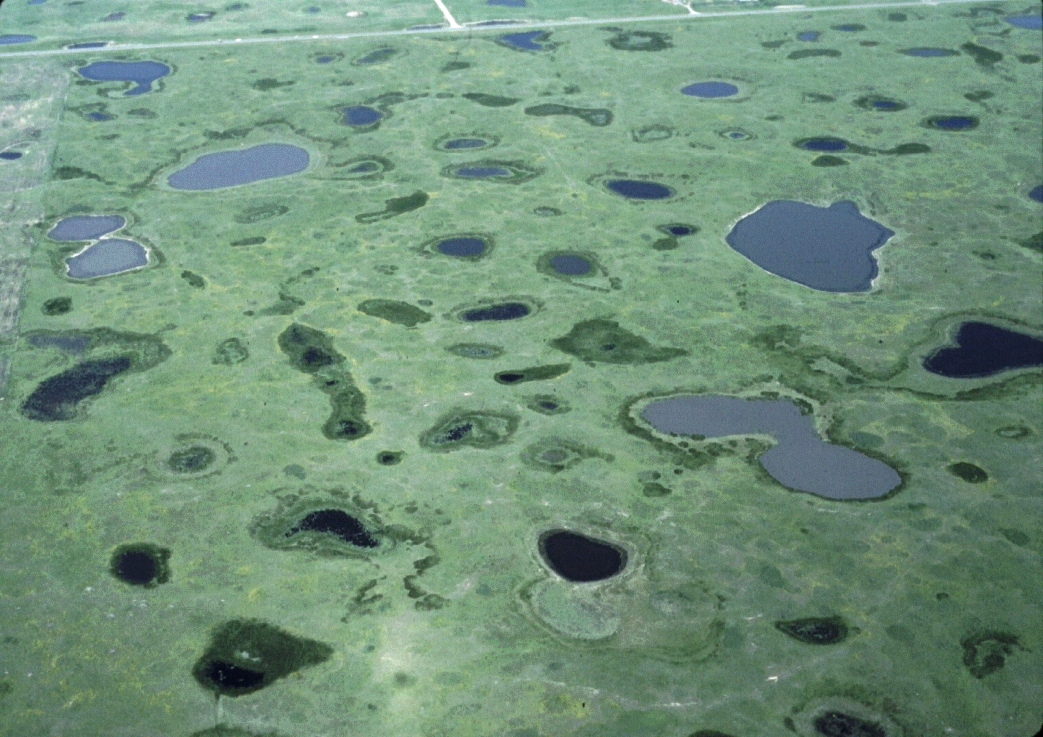
\includegraphics[width=\textwidth]{figs/Prairie_Pothole_Wetlands}
  \end{center}
\end{frame}





\begin{frame}
  \frametitle{Single-season model}
  \large
  {\centering Model for the occurrence state}
  \[
    O_{i} \sim \mbox{Bernoulli}(\psi)
  \] \\
  \pause
  \vspace{0.4cm}
  {\centering Model for the data}
  \[
    y_{ij} \sim \mbox{Bernoulli}(O_i \times p)
  \] \\
  \pause
  \vspace{0.5cm}
  We need to estimate $\psi$ (occurrence probability) and $p$ (detection probability)
\end{frame}





\begin{frame}
  \frametitle{Design}
  \large
  To estimate $\psi$ and $p$, we should use a good study design:
  \begin{itemize}[<+->]
    \item We need multiple sites
    \item Sites should be randomly selected
    \item We must have multiple sampling occasions at (a subset of) the sites
%    \item Determining how many sites and occasions depends on $\psi$ and $p$
  \end{itemize}
\end{frame}






\begin{frame}
  \frametitle{Data $y_{ij}$ -- low detection probability}
  {%\bf
    \centering \large 10 sites and 3 sampling occasions \par}
  \vspace{0.3cm}
  \begin{center}
    \small
    \begin{tabular}{lccc}
      \hline
      & Occasion 1 & Occasion 2 & Occasion 3 \\
      \hline
      Site 1 & 0 & 0 & 1 \\
      Site 2 & 0 & 0 & 0 \\
      Site 3 & 0 & 0 & 0 \\
      Site 4 & 1 & 0 & 0 \\
      Site 5 & 0 & 0 & 0 \\
      Site 6 & 1 & 0 & 1 \\
      Site 7 & 1 & 0 & 0 \\
      Site 8 & 0 & 0 & 0 \\
      Site 9 & 0 & 1 & 0 \\
      Site 10 & 0 & 0 & 0 \\
      \hline
    \end{tabular}
  \end{center}
%  \pause
%  Naive occupancy = 5/10 = 0.50 \\
%  Estimated occupancy = $\hat{\psi} = 0.61$
\end{frame}





\begin{frame}
  \frametitle{Data $y_{ij}$ -- high detection probability}
  {%\bf
    \centering \large 10 sites and 3 sampling occasions \par}
  \vspace{0.3cm}
  \begin{center}
    \small
    \begin{tabular}{lccc}
      \hline
      & Occasion 1 & Occasion 2 & Occasion 3 \\
      \hline
      Site 1 & 1 & 1 & 1 \\
      Site 2 & 0 & 0 & 0 \\
      Site 3 & 0 & 0 & 0 \\
      Site 4 & 1 & 1 & 1 \\
      Site 5 & 0 & 0 & 0 \\
      Site 6 & 1 & 0 & 1 \\
      Site 7 & 1 & 1 & 1 \\
      Site 8 & 0 & 0 & 0 \\
      Site 9 & 0 & 1 & 1 \\
      Site 10 & 0 & 0 & 0 \\
      \hline
    \end{tabular}
  \end{center}
%  \pause
%  Naive occupancy = 5/10 = 0.50 \\
%  Estimated occupancy = $\hat{\psi} = 0.61$
\end{frame}






\begin{frame}
  \frametitle{How do we estimate $\psi$ and $p$?}
  \pause
  \begin{columns}
    \begin{column}{0.6\textwidth}
      \large {%\bf
        Maximum likelihood \par}
      \large
      \begin{itemize}%[<+->]
      \item This method tries to find the most ``likely'' values of
        $\psi$ and $p$, given the data
      \item It can also be used to estimate standard errors (SEs) and
        confidence intervals (CIs)
      \end{itemize}
    \end{column}
    \pause
    \begin{column}{0.4\textwidth}
      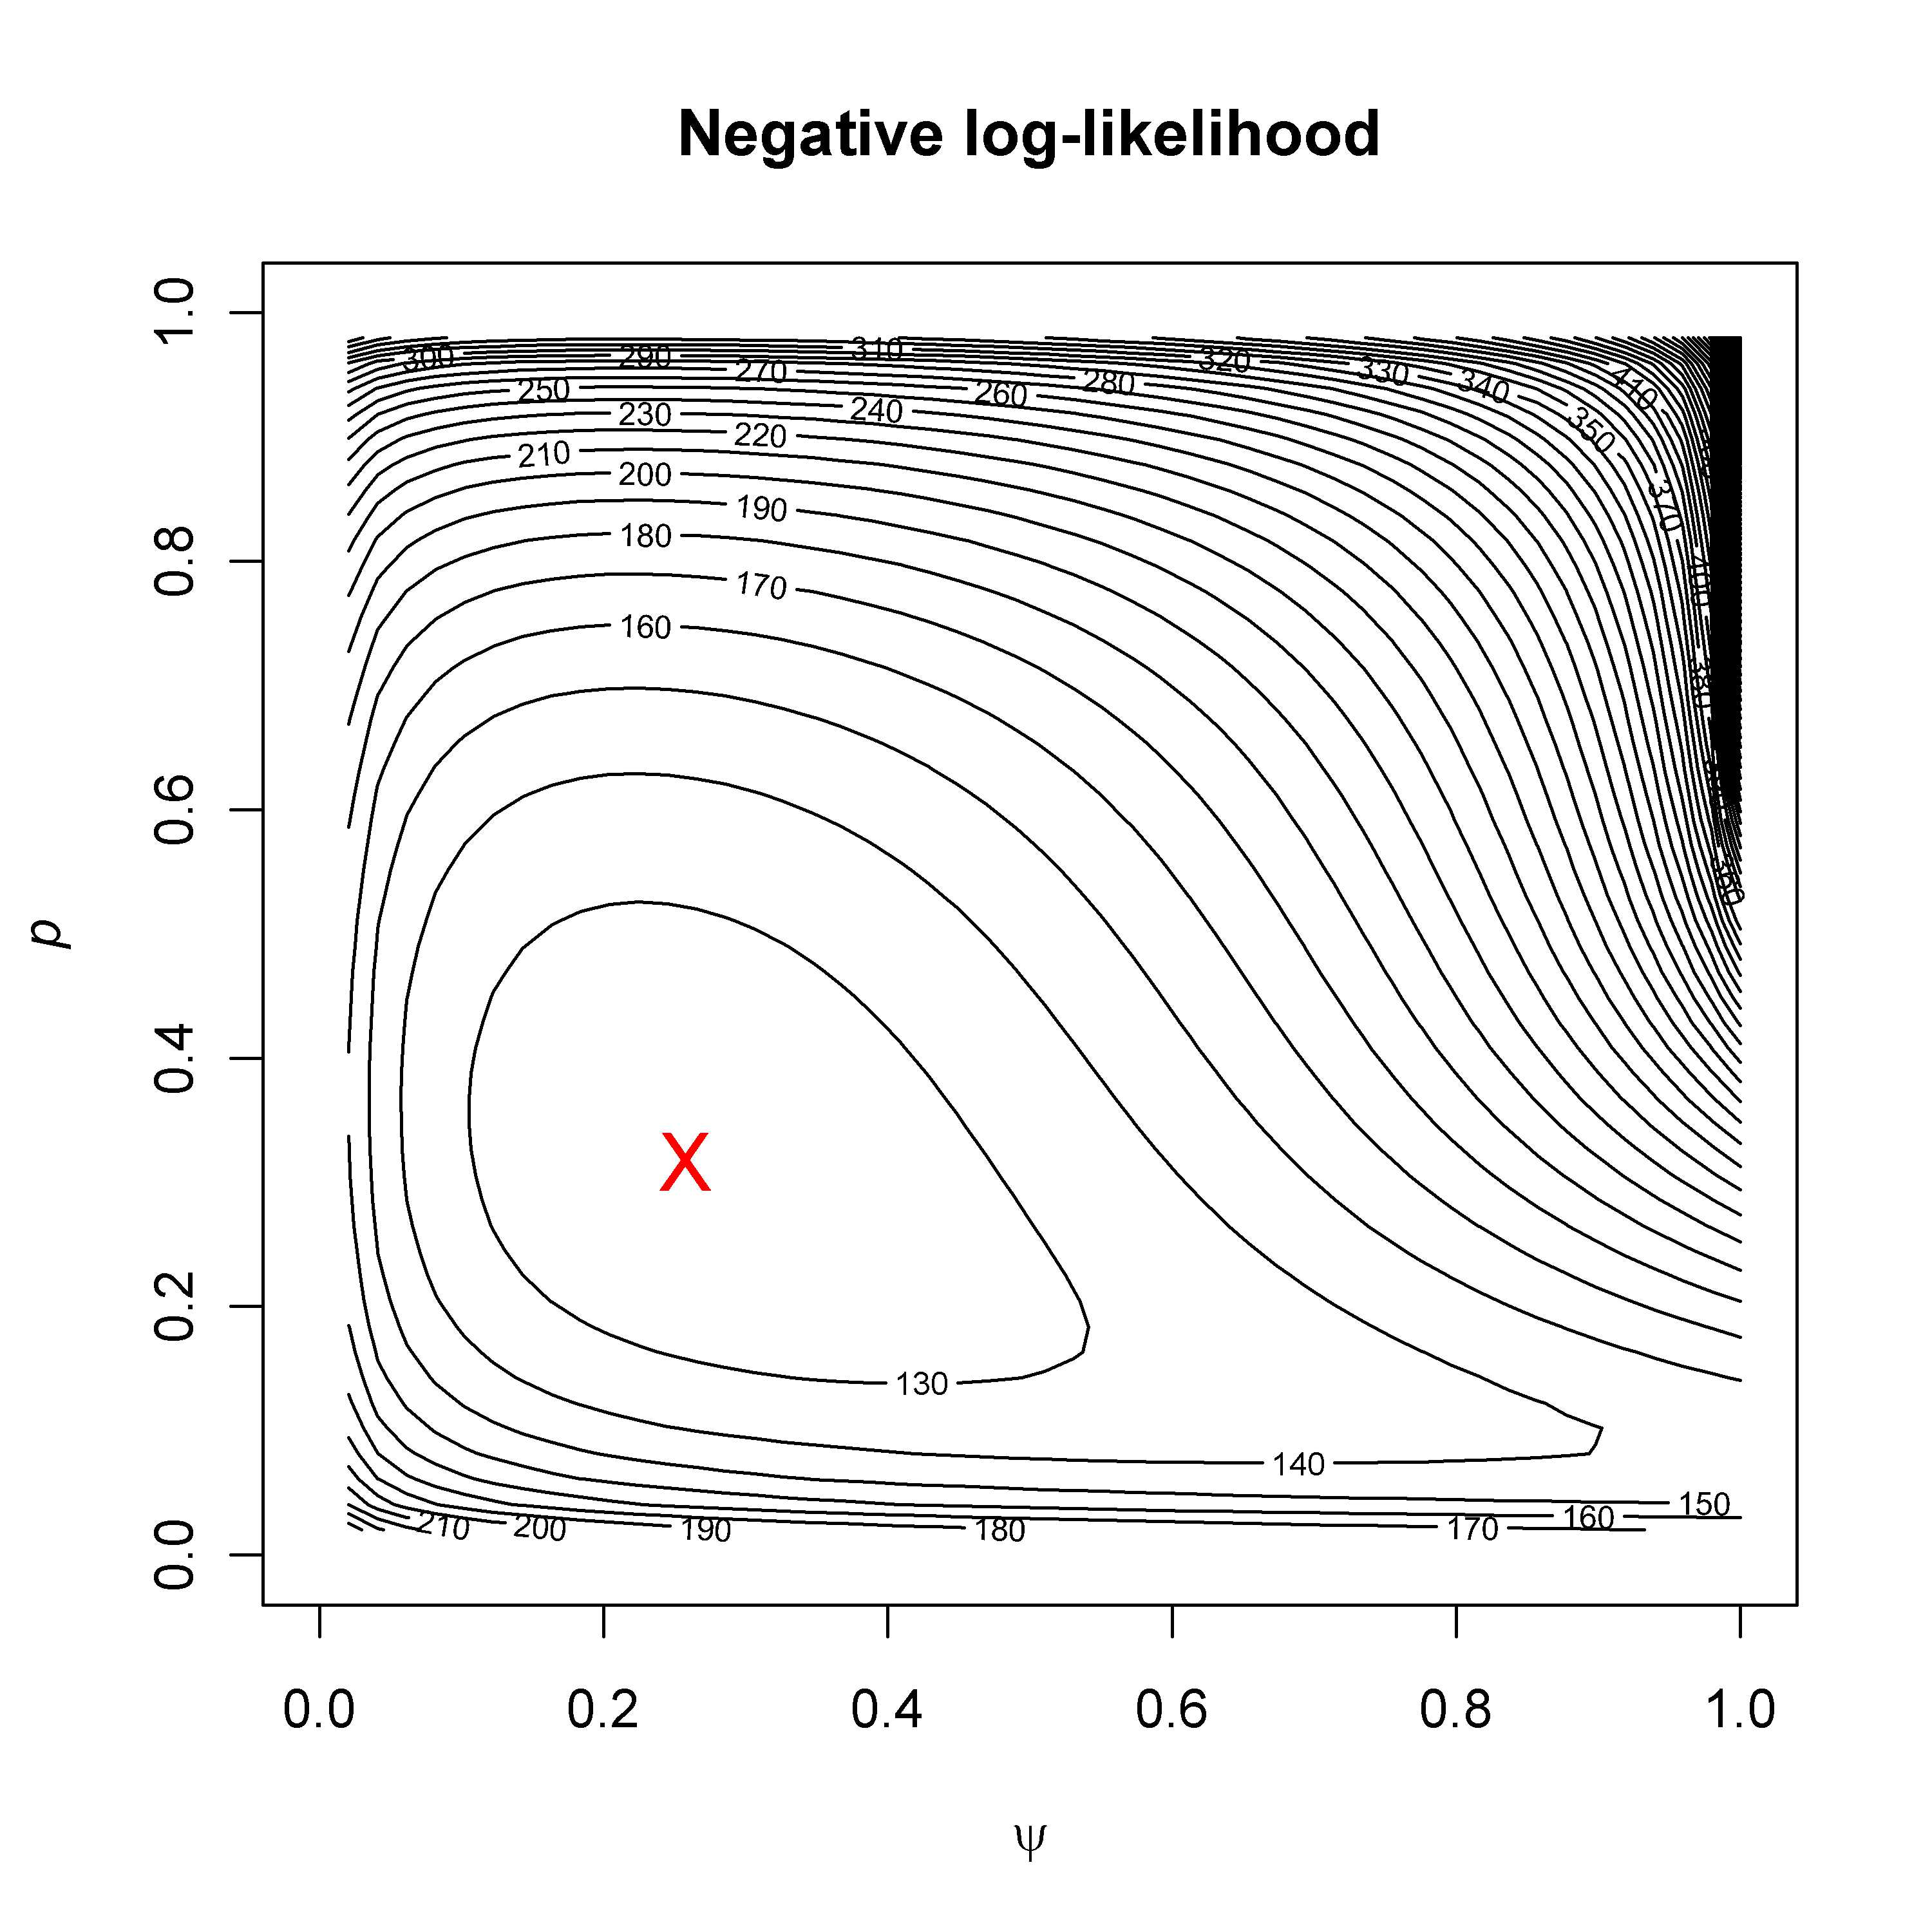
\includegraphics[width=\textwidth]{figs/mlePandPsi}
    \end{column}
  \end{columns}
  \pause
  {%\bf
    Software \par}
  Program {\tt PRESENCE}, Program {\tt MARK}, {\tt R} package {\tt unmarked}
\end{frame}




\begin{frame}
  \frametitle{Estimates}
  {%\bf
    \centering \large 10 sites and 3 sampling occasions \par}
  \vspace{0.3cm}
  \begin{center}
    \small
    \begin{tabular}{lccc}
      \hline
      & Occasion 1 & Occasion 2 & Occasion 3 \\
      \hline
      Site 1 & 0 & 0 & 1 \\
      Site 2 & 0 & 0 & 0 \\
      Site 3 & 0 & 0 & 0 \\
      Site 4 & 1 & 1 & 0 \\
      Site 5 & 0 & 0 & 0 \\
      Site 6 & 1 & 1 & 1 \\
      Site 7 & 1 & 0 & 0 \\
      Site 8 & 0 & 0 & 0 \\
      Site 9 & 0 & 1 & 0 \\
      Site 10 & 0 & 0 & 0 \\
      \hline
    \end{tabular}
  \end{center}
%  \pause
  Naive occupancy = 5/10 = 0.50 \\
  Estimated occupancy = $\hat{\psi} = 0.61 \pm 0.22$ \\
  Estimated detection = $\hat{p} = 0.44 \pm 0.16$ \\
\end{frame}




\begin{frame}
  \frametitle{Overall detection probability}
  \large
  {\centering If you sample a site $K$ times, the overall detection
    probability ($\bar{p}$) is:}
  \[
    \bar{p} = 1 - (1-p)^K
  \]
  \vfill
  \large
  $\bar{p}$ is detection probability after $K$ sampling occasions \\
  $p$ is detection probability on a single occasion \\
  $K$ is the number of sampling occasions (e.g., visits to a site)
\end{frame}









\begin{frame}
  \frametitle{Assumptions}
  \large
  \begin{enumerate}[<+- | visible@+->][\bf \color{PineGreen} (1)]
    \item Population closure: Occurrence state does not change during sampling
    \item Occurrence probability is the same for all sites, unless we
      account for \alert{covariates}
    \item Detection probability is the same for all sites and sampling
      occasions, unless we account for covariates
    \item Statistical independence
  \end{enumerate}
\end{frame}



\begin{frame}
  \frametitle{Covariates}
  \large
  The value of $\psi$ or $p$ may depend on other variables,
  e.g. habitat, weather, observer abilities \\
%  \begin{itemize}
%    \item Habitat
%    \item Weather
%    \item Observer abilities
%  \end{itemize}
  \pause
  \vspace{0.4cm}
  How do we accommodate covariates? \\
  \pause
  \vspace{0.4cm}
  The key is to think of detection probability as a function. A common
  choice is the logit-linear model:
  \[
    \mbox{logit}(\psi_i) = \beta_0 + \beta_1\mbox{ELEV}_i
  \]
\end{frame}












\begin{frame}[fragile]
  \frametitle{Covariates}
  \begin{center}

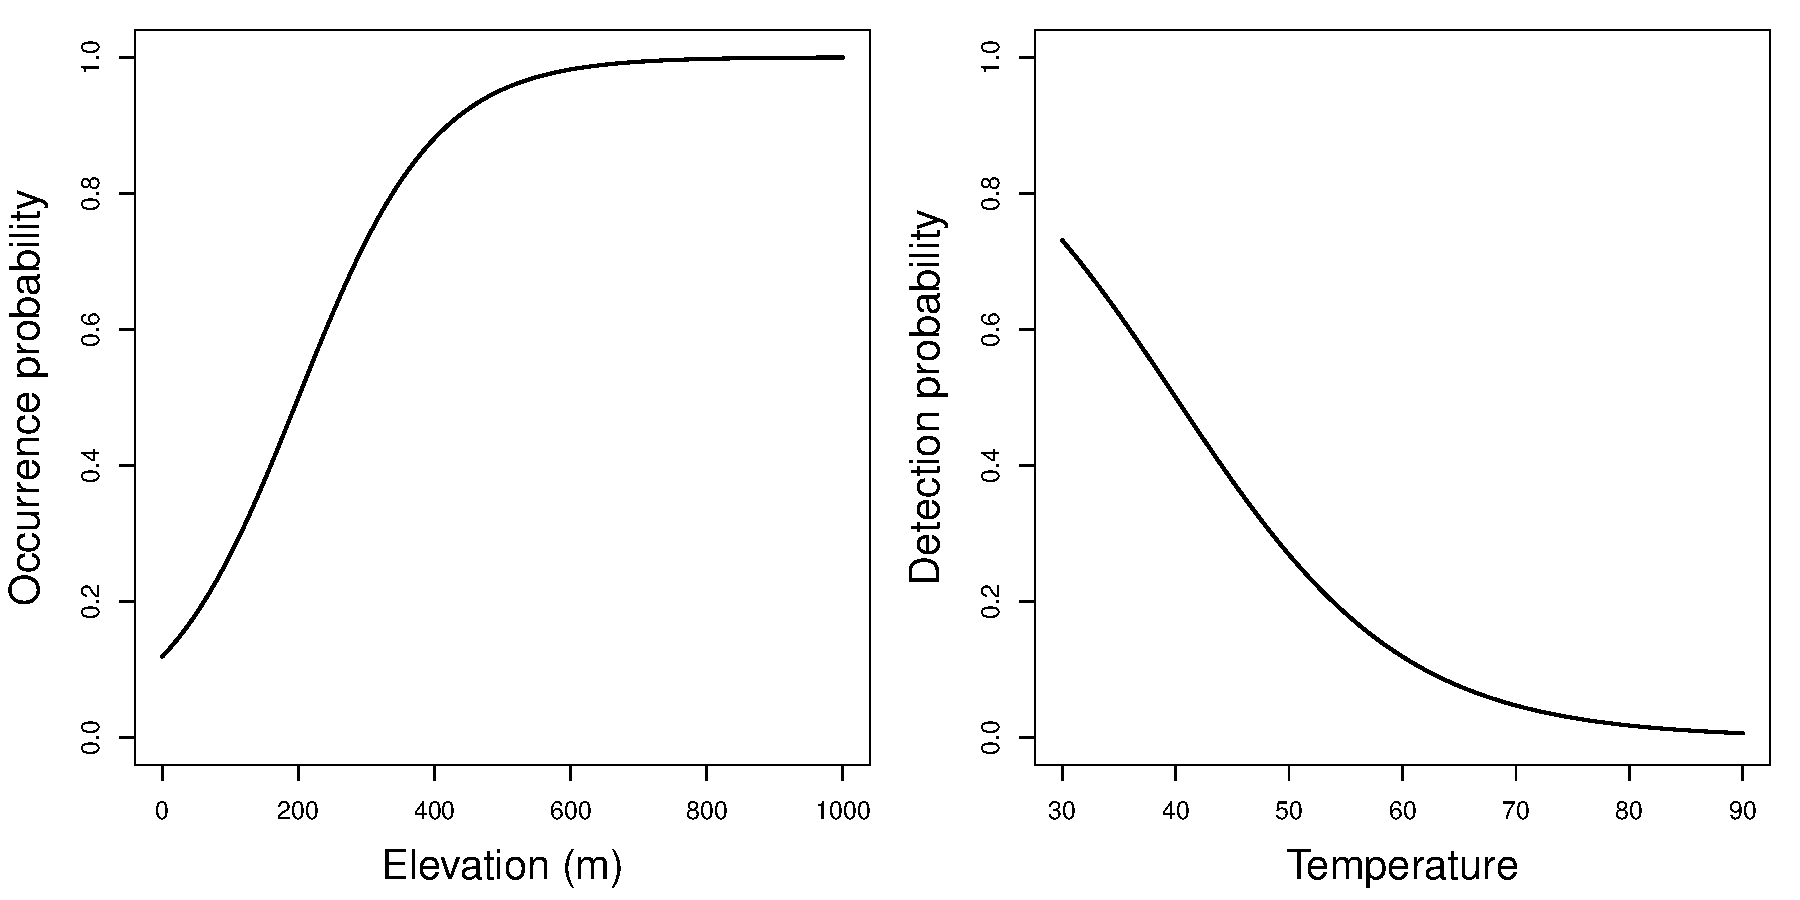
\includegraphics[width=\textwidth]{figs/cov1}
  \end{center}
\end{frame}






\section{Multi-season models}



\begin{frame}
  \frametitle{Multi-season models}
  \large
  With more than 1 season, we can estimate all the parameters of our
  metapopulation model, plus detection probability $p$
  \pause
  \[
    \psi_{i,t+1} = O_{i,t}(1-\varepsilon) + (1-O_{i,t})\gamma
  \]
  \[
    O_{i,t+1} \sim \mbox{Bernoulli}(\psi_{i,t+1})
  \]
  \[
    y_{i,j,t} \sim \mathrm{Bernoulli}(O_{i,t} \times p)
  \]
\end{frame}




\begin{frame}
  \frametitle{Data format}
  {%\bf
    \centering \large 5 sites, 2 seasons, and 3 sampling occasions \par}
  \vspace{0.3cm}
  \begin{columns}
%    \begin{center}
    \column{\dimexpr\paperwidth-10pt}
%      \tiny
    \scriptsize
      \begin{tabular}{lccccccc}
        \hline
        & \multicolumn{3}{c}{Season 1} & &
        \multicolumn{3}{c}{Season 2} \\
        \cline{2-4} \cline{6-8}
        & Occasion 1 & Occasion 2 & Occasion 3 & & Occasion 1 & Occasion 2 & Occasion 3 \\
        \hline
        Site 1 & 0 & 0 & 1 & & 1 & 0 & 0 \\
        Site 2 & 0 & 0 & 0 & & 0 & 0 & 0 \\
        Site 3 & 0 & 0 & 0 & & 1 & 0 & 0 \\
        Site 4 & 1 & 1 & 1 & & 0 & 0 & 0 \\
        Site 5 & 0 & 0 & 0 & & 1 & 1 & 0 \\
        \hline
      \end{tabular}
%    \end{center}
  \end{columns}
\end{frame}




\begin{frame}
  \frametitle{Summary}
  \large
  Occupancy models let us estimate metapopulation parameters
      when detection is imperfect. 
  \pause
  \vfill
  There are no individual-level data or parameters.
  \pause
  \vfill
  These methods are often easy to implement over large areas
  and so are used in monitoring programs. 
  \pause
  \vfill
  Definition of site and season are very important considerations. 
  \pause
  \vfill
  Models can be used in other contexts, such as when a site is
  a human, and we are interested in proportion of people with some disease. 
\end{frame}



%% \section{Software}


%% \begin{frame}
%%   \frametitle{Program {\tt PRESENCE}}
%%   Need to provide guideance for lab
%% \end{frame}




%% \begin{frame}
%%   \frametitle{{\bf R} Package {\tt unmarked}}
%%   Need to provide guideance for lab
%% \end{frame}



\end{document}
